\glsresetall % reset all the acronyms
\chapter{Efficient High-SNR Signal Acquisition}\label{ch:cft}
This chapter focuses on the first stage of radar-based ECG recovery to acquire high-SNR radar signals with ample cardiac features, because the quality of the radar inputs highly affects the fidelity of ECG recovery~\cite{chen2022contactless,zhang2024radarODE}. Previous methods either require traversing a large search space to extract high-SNR signal or applying signal accumulation to suppress constant noises and enhance cardiac features, causing massive demand on computational resources and only applicable to short-range monitoring. In this chapter, a novel algorithm called \gls{cft} is proposed to find the \gls{cf} point by iteratively evaluating the potential points in a discontinuous objective space, and the CFT algorithm is tested on the sitting subjects to provide radar measurements with better SNR compared with existing methods.

\section{Introduction}
\Gls{radar} system is originally designed for military detection of large aircraft by emitting electromagnetic waves and evaluating the reflections. The follow-up research has investigated the civilian use of radar systems for contactless sensing in various scenarios, such as autonomous driving~\cite{yao2023waterscenes} and human monitoring~\cite{zhang2023overview}. Over the past decade, radar-based sensing has been empowered by deep neural networks to process non-stationary reflected signals or high-dimensional data, enabling versatile applications to replace contact- or visual-based measurement for convenience or privacy concerns (e.g., vital sign monitoring~\cite{liu2024diversity}, gesture recognition~\cite{song2025dual}, fault diagnosis~\cite{chen2024two}).

Radar-based vital sign monitoring, as a popular branch of radar-based sensing, has been explored for decades to measure heart rate or respiration rate in a contactless manner~\cite{zhang2023overview}, and some further studies leverage the deep neural network to realize domain transformation from cardiac mechanical activities (i.e., heartbeat) to electrical activities (i.e., ECG), providing a fine-grained cardiac measurement for wellness monitoring or clinical diagnosis~\cite{zhao2024mmarrhythmia,zhang2024radarODE,zhang2024radarODE-MTL,chen2022contactless,zhang2025horcrux,li2024radarnet,wu2023contactless}. In the literature, radar-based ECG recovery is only realized by deep-learning-based methods, because the domain transformation is extremely complex to be modeled mathematically while such transformation can be learning by deep learning model due to the great nonlinear mapping ability~\cite{chen2022contactless}.

\begin{figure}[tb]
        \centering
        \subfloat[]{\label{fig:radar_good}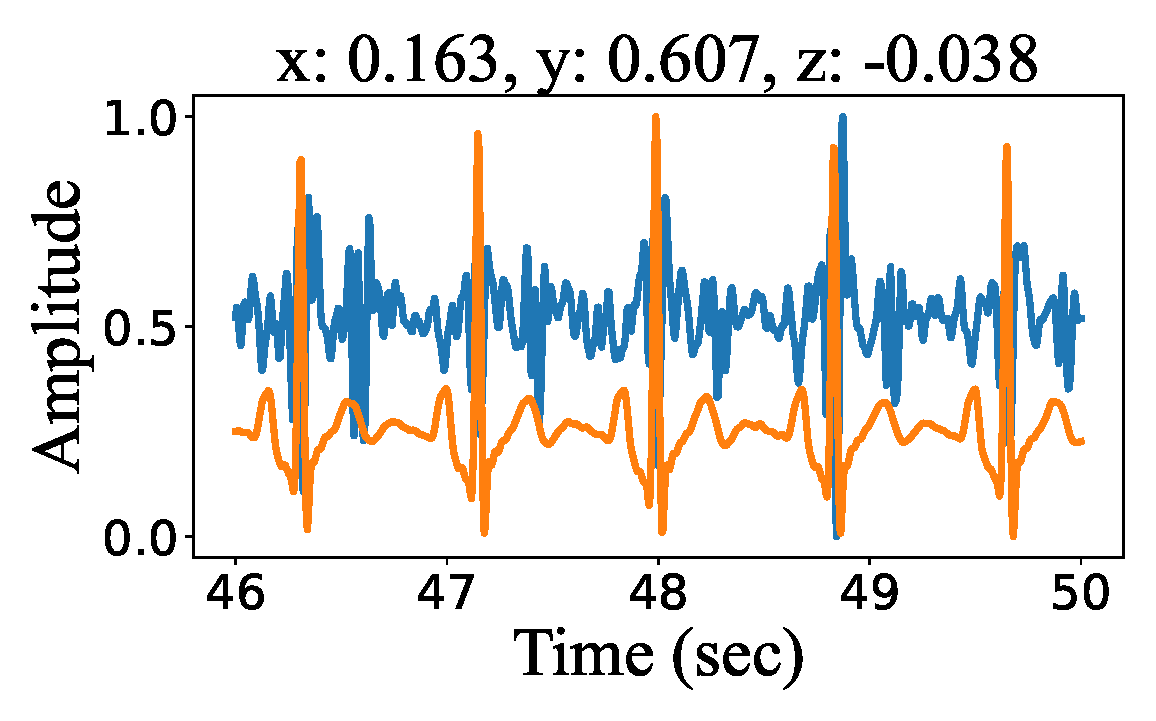
\includegraphics[width=0.35\columnwidth]{radar_good.eps}}
        \subfloat[]{\label{fig:radar_bad}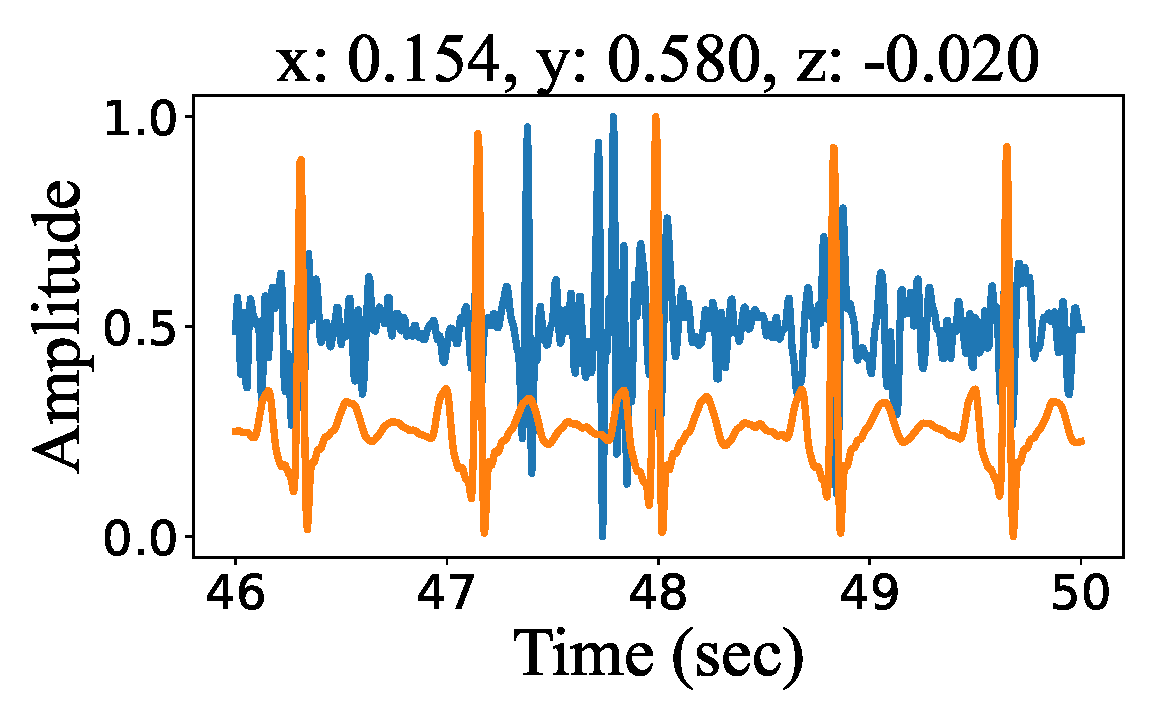
\includegraphics[width=0.35\columnwidth]{radar_bad.eps}} 
        \caption{Challenges for high-SNR signal collection: (a) and (b) Radar signals with high and low SNR for adjacent points with a distance of $0.03$m.}
        \label{fig:challenges}
\end{figure}
Based on the discussion Chapter~\ref{sec:the_first_challenge}, it is still a challenge to precisely locate and track the cardiac location during data collection to efficiently extract high-SNR radar signal. Although, it is natural to think the high-SNR radar signal can be searched in a constrained space by optimization, there is no appropriate method to assess the signal SNR in terms of cardiac features contained, and the objective space is actually highly discontinuous with adjacent points may revealing totally different SNR as shown in Figure~\subref*{fig:radar_good} and~\subref*{fig:radar_bad}, restricting the application of common gradient-based optimization algorithms. To address these issues, the contributions of this study can be listed as: 
\begin{itemize}
\item A \gls{cft} algorithm is proposed based on derivative-free optimization (DFO) to find the gls{cf} point by iteratively evaluating the potential points in a discontinuous objective space, with a universal signal template designed to adaptively assess the signal SNR as costs.
\item The proposed CFT algorithm has been validated on sitting subjects in various scenarios and could provide radar measurements with better SNR compared with existing methods.
\end{itemize}

The rest of this chapter is organized as follows. Section~\ref{sec:cftmethod} elaborates the proposed CFT algorithm, with the experimental settings and results shown in Section~\ref{sec:cftexp} and~\ref{sec:cftresult}. The final conclusion is shown in Section~\ref{sec:cftcon}.


\section{Methodology}\label{sec:cftmethod}
\subsection{Overview of CFT Algorithm for ECG Recovery}
The pipeline of using CFT algorithm is shown in Figure~\ref{fig:CFTRFcardi} with three steps:
\begin{itemize}
\item The received radar signal will be converted into a standard format in terms of chirp, frame and virtual antenna channel to obtain the general location of the subject, as shown in Figure~\ref{fig:CFTRFcardi}(a).
\item The rough location acts as the initial state for the CFT algorithm, and the points within a constrained space will be evaluated to find the red CF point with best SNR as shown in Figure~\ref{fig:CFTRFcardi}(b).
\item Signals extracted from the ten best points will be converted into spectrograms to train the deep learning model designed in~\cite{zhang2024radarODE-MTL} and generate corresponding ECG recoveries, as shown in Figure~\ref{fig:CFTRFcardi}(c).
\end{itemize}

In addition, TI-AWR 1843 radar operated at $77$~Ghz with $2$~Tx and $4$~Rx will be used for data collection, enabling $8$ virtual antenna channels for high-quality signal extraction. The detailed scenario descriptions and radar configurations will be provided in Section~\ref{sec:cftdata_coll}.

\begin{figure}[tb] 
    \centering 
    \includegraphics[width=0.99\columnwidth]{CF_Cardi_struct.pdf}
    \caption{Overview of using CFT for radar-based ECG covery: (a) Rough localization of human body; (b) Use CFT to find CF point and extract high-SNR radar signals; (c) Deep learning for ECG recovery.}
    \label{fig:CFTRFcardi} 
\end{figure}

\subsection{Rough Localization}
The received radar signal is first formatted as a standard data matrix in terms of different chirps, frames and virtual channels to provide measurement of range, velocity and AoA, respectively. For the current research level of radar-based vital sign monitoring, the subjects are all quasi-static without velocity, and only the range-angle (RA) map will be calculated using fast Fourier transform (FFT) as shown in Figure~\ref{fig:CFTRFcardi}(a), with a detailed illustration of signal waveform and processing shown in Figure~\ref{fig:rouch_loc}.

\subsubsection{Range FFT}
According to (\ref{equ:raw_sig}), the signal propagation after transmitting introduces a constant phase shift $\phi_s$ in the received signal and is expressed as 
\begin{equation}\label{equ:range}
\phi_s = \frac{4\pi d_0}{\lambda}
\end{equation}
with $d_0$ representing the distance between radar and human body. Therefore, the distance $d_0$ can be extracted from each received signal along fast time using FFT as shown in Figure~\ref{fig:rouch_loc}(a), and the updated data matrix now reveals the range information, i.e., a static object denoted as blue along slow time axis.
\begin{figure}[tb] 
    \centering 
    \includegraphics[width=0.9\columnwidth]{rough_loc.pdf}
    \caption{Procedures for obtaining RA map: (a) Range FFT for chirps along fast time; (b) Angle FFT along virtual channels.}
    \label{fig:rouch_loc} 
\end{figure}
\subsubsection{Angle FFT}
The ability of AoA detection relies on the MIMO system using time division multiplexing (TDM-MIMO), with multiple Tx alternately transmitting chirp signals and the corresponding reflections can be distinguished during receiving as shown in Figure~\ref{fig:rouch_loc}(b). Due to the physical distance varies for different Tx/Rx combinations (i.e., Tx$2$Rx$4$ creates $8$ virtual channels), an extra propagation $\Delta \phi_v$ delay will be introduced as:
\begin{equation}\label{equ:angle}
\begin{aligned}
\Delta \phi_v &= \frac{4\pi d_v}{\lambda} \\
d_v &= l\ sin(\theta)
\end{aligned}
\end{equation}
where $d_v$ represents the extra propagation distance, $l$ means the distance between adjacent antenna channels and $\theta$ is the incident angle. Similar to range FFT, the phase differences across different channels can be used to extract AoA information for each range bin by performing FFT along the channel axis, as shown in red squares in Figure~\ref{fig:rouch_loc}(b).

After combining the FFT results for all chirps and channels, the final RA map for the current time sample (frame) can be obtained as shown in Figure~\ref{fig:rouch_loc}. The same procedure can be repeated along the slow time axis to get the rough human body location for all the time samples, but this study only requires the location obtained from the very first frame as the initial point $E_0$ for CFT algorithm.

\subsection{Cardio-focusing and -tracking (CFT) Algorithm}
The radar signal for any point can be extracted following (\ref{equ:raw_sig}) and (\ref{equ:phase}), and the search progress from $E_0$ to the best point $E_{b}$ (i.e., CF point with high SNR) requires: (a) an appropriate metric to assess whether the radar signal contains wanted cardiac features; (b) an optimization method that is applicable to the discontinuous objective space based on the assessed SNR values as costs. 

\subsubsection{Template Design for Assessing SNR}
An explicit SNR can be calculated with the known “clean” signal, while the "clean" signal for vital signs normally reveals two prominent vibrations corresponding to the ventricular contraction and relaxation~\cite{zhang2024radarODE}, as shown in Figure~\subref*{fig:target_org}. However, considering the vibrations may have subtle differences due to different scenarios or radar configurations (e.g., noise figure and sampling frequency), a universal template $h_m$ is designed in this study to fit the envelope of the radar signal as: 
\begin{equation}
h_m (t) = a_1 \exp(-\frac{(t-b_1)^2}{2c_1^2}) + a_2 \exp(-\frac{(t-b_2)^2}{2c_2^2})
\end{equation}
with $a_1$, $a_2$ controlling the amplitudes of the peaks, $b_1$, $b_2$ determining the centers of the peaks and $c_1$, $c_2$ adjusting the width of the peaks. In practice, $a_1$ and $b_1$ will be fixed based on the dominant peaks detected as the red points in Figure~\subref*{fig:target_sig}, and other parameters are left to be determined as a simple curve fitting problem. Finally, the \gls{mse} between the radar signal envelope and the synthetic template is reckoned to be an assessment of signal SNR as shown in Figure~\subref*{fig:target_sig}, because fewer components could fit the designed template for low-SNR radar signal without obvious cardiac features, as shown in Figure~\subref*{fig:target_org_bad} and~\subref*{fig:target_sig_bad}.

\begin{figure}[tb]
  \centering
  \subfloat[]{\label{fig:target_org}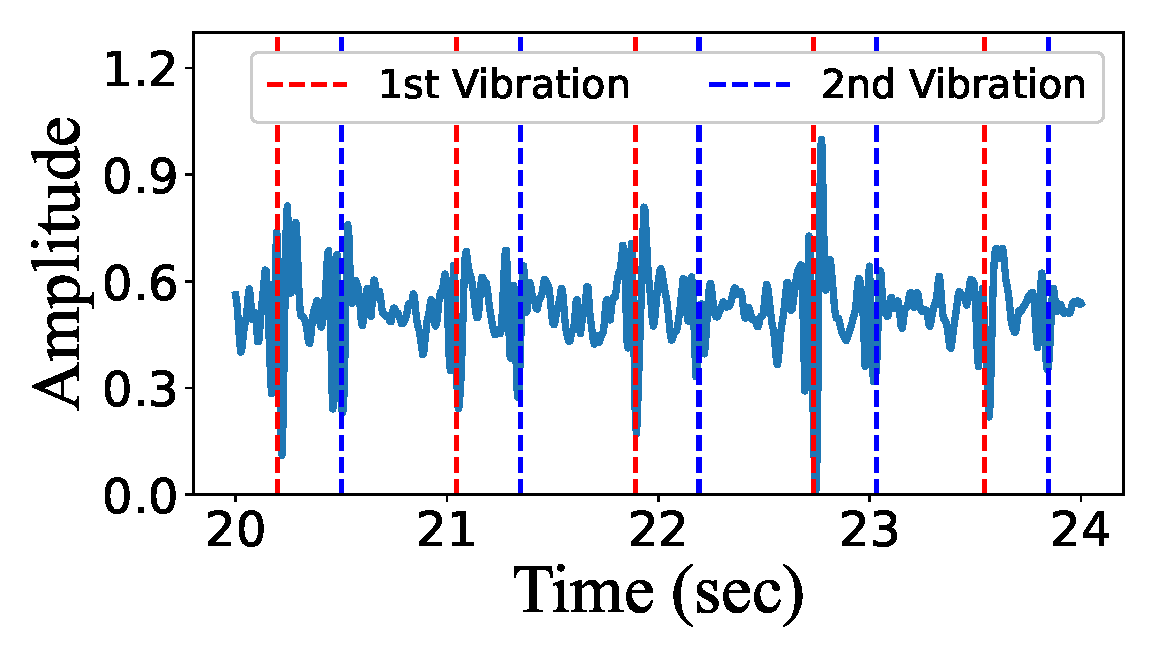
\includegraphics[width=0.4\columnwidth]{target_org.eps}}
  \subfloat[]{\label{fig:target_sig}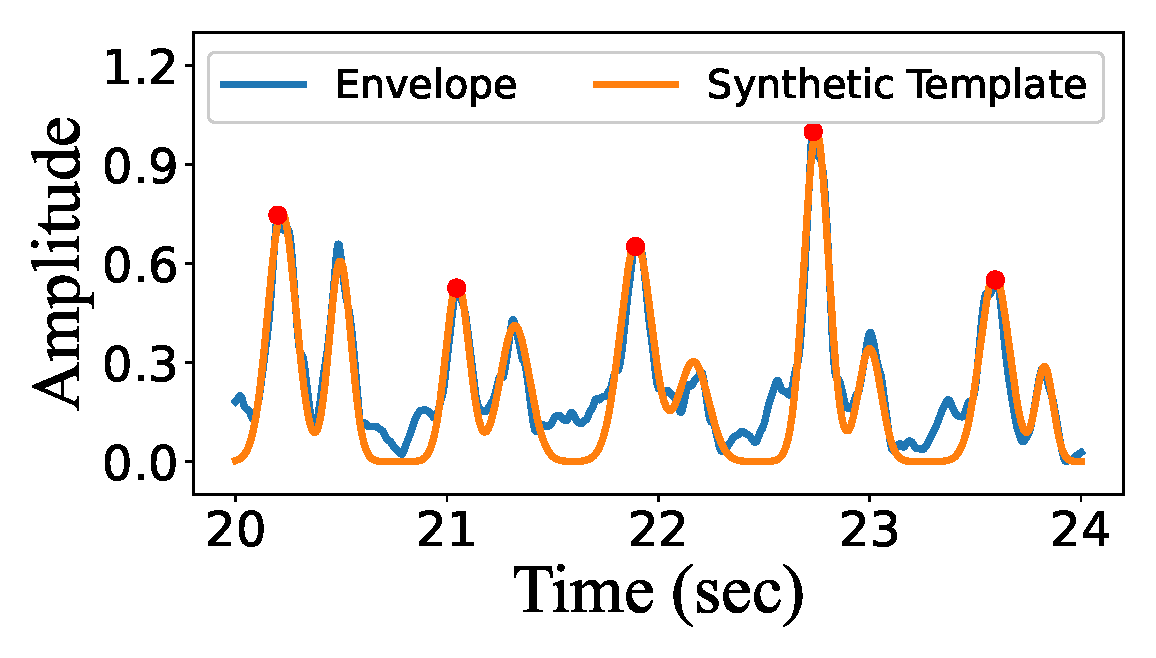
\includegraphics[width=0.4\columnwidth]{target_sig.eps}} \\
  \subfloat[]{\label{fig:target_org_bad}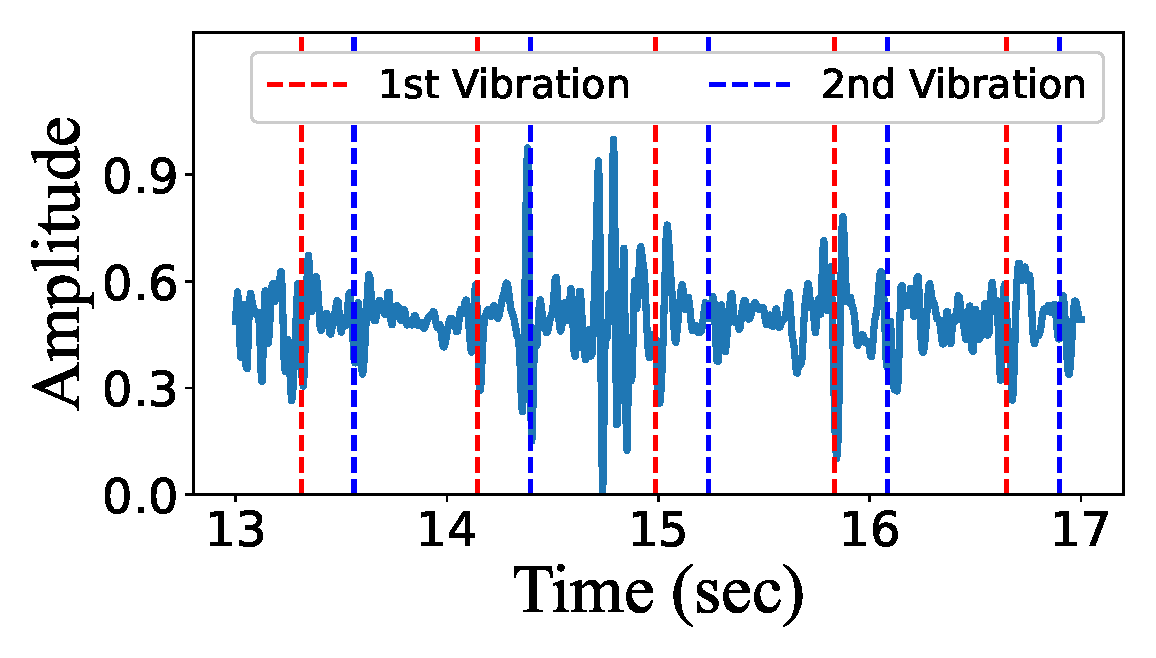
\includegraphics[width=0.4\columnwidth]{target_org_bad.eps}}
  \subfloat[]{\label{fig:target_sig_bad}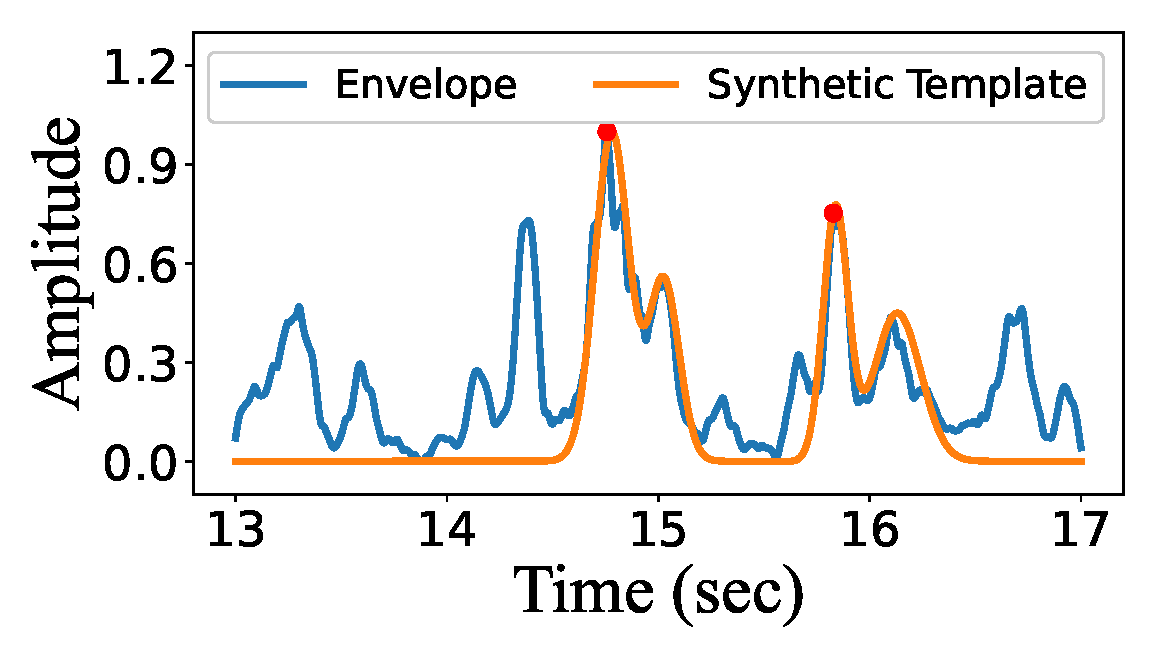
\includegraphics[width=0.4\columnwidth]{target_sig_bad.eps}}
  \caption{Template for assessing SNR: (a) High-SNR radar signal; (b) Extracted signal envelope with the synthetic template; (c) (a) Low-SNR radar signal, (d) Extracted signal envelope with the synthetic template.}
  \label{fig:template}
\end{figure}

\subsubsection{Derivative-free Optimization (DFO)}
The MSE values obtained from template matching for the radar pieces extracted from point $E$ will be used as costs $\mathcal{F}(E)$ in searching CF point, but the traditional gradient-based optimization method is not applicable because there is no explicit cost function. Therefore, the CFT algorithm is developed in a derivative-free manner based on coordinate search (CS) algorithm~\cite{larson2019derivative}, to asymptotically approach the CF point. 

The definition of the DFO problem is formulated as:
\begin{equation}
E_b = \underset{E \in \mathbb{R}^n}{\arg \min }\left\{\mathcal{F}(E) : E\in \Omega \right\}
\end{equation}
with $\Omega$ representing a user-defined constrained $n$-dimensional search space near initial point $E_0$ as shown in Figure~\ref{fig:CFTRFcardi}(b), and the cost of points out of the constraint will be set as $\mathcal{F}(E\not\in \Omega)=\infty$. During each iteration $k$, many trial points $E_k$ within the constraint will be evaluated to find the incumbent points $E_i$ as the temporary best point for the next iteration. 

To perform a derivative-free search, the traditional CS algorithm starts from the initialization of grids $G_k$:
\begin{equation}\label{equ:grid}
G_k := \{E_k + \gamma_kD\} \subset \mathbb{R}^n
\end{equation}
where $\gamma_k>0$ is the grid size parameter and $D$ contains several vectors $p$ for possible searching directions, as shown in Figure~\subref*{fig:cft_1}. The local convergence of CS is ensured by dense search directions $D$ and a refined grid size $\gamma_k$ to find better $E_i$ compared with current $E_k$~\cite{larson2019derivative}. However, the highly discontinuous objective space for radar-monitored vital signs may have numerous local minima that distract the optimization algorithm, i.e., the signal SNR of the adjacent points might be very different, as shown in Figure~\subref*{fig:radar_good} and~\subref*{fig:radar_bad}.

\begin{figure}[tb]
  \centering
  \begin{minipage}[t]{0.5\columnwidth}
  \subfloat[]{\label{fig:cft_1}\includegraphics[width=0.5\columnwidth]{cft_1.pdf}}\\
  \subfloat[]{\label{fig:cft_2}\includegraphics[width=0.5\columnwidth]{cft_2.pdf}}
  \end{minipage}%
  \hspace{-0.2\columnwidth}
  \begin{minipage}[t]{0.5\columnwidth}
  \vspace{0.08\columnwidth}
  \subfloat[]{\label{fig:cft_3}\includegraphics[width=1\columnwidth]{cft_3.pdf}}
  \end{minipage}%
  \caption{Illustration of the CFT algorithm with bold line wrapping the search region $S_k$: (a) Equality between $\gamma$ and $\Gamma$ (same as in CS algorithm); (b) Large $\Gamma_k$ with refined $\gamma_k$, providing more potential points to be evaluated; (c) Jump out of the local minimum by adjusting $\Gamma_k$ and $\gamma_k$.}
  \label{fig:cft_plot}
\end{figure}

To jump out of the potential local minimum, CFT algorithm is proposed by introducing search region $S_k$ to restrict the possible search directions $p$, alleviating the difficulty of searching in numerous dense grid points and allowing the adjustment of search region and grid size iteratively to break the local minimum. The detailed procedures of CFT are shown in Algorithm~\ref{alg:CFT}, with an illustration of $\mathbb{R}^2$ space shown in Figure~\ref{fig:cft_plot}. 

In CFT, the grids $G_k$ is still expressed as in (\ref{equ:grid}) and the newly introduced search region $S_k$ is expressed as:
\begin{equation}
S_k := \{E\in G_k : \| E-E_k \|_{\infty} \leq \Gamma_k a \}
\end{equation}
with $a=\max \left\{\left\|a^{\prime}\right\|_{\infty}: a^{\prime} \in D\right\}$ and $\Gamma_k$ as the size parameter for the search region. An intuitive interpretation of $S_k$ is the point set that contains grid points inside and on the boundary of the bold line controlled by $\Gamma_k$, as shown in Figure~\subref*{fig:cft_2}.

Based on the well-constructed grids $G_k$ and search region $S_k$, the remaining CFT algorithm is performed with searching and resizing stages:

\textbf{Searching: } The searching stage simply asks for the evaluation of $\mathcal{F}(E)$ on a subset of grids $G_k$ based on any sampling algorithm (e.g., Latin hypercube sampling~\cite{larson2019derivative}), as indicated in line~\ref{line:s1} in Algorithm~\ref{alg:CFT}.

\textbf{Resizing: } The resizing stage depends on the result of searching stage: 
\begin{itemize}
  \item If a new incumbent point $E_i$ is found with better SNR, the search region will be doubled as $\Gamma_{k+1}=2\Gamma_k$ (line~\ref{line:r1}), and the grid size will be empirically set as $\gamma_{k+1}=\min(\Gamma_k, {\Gamma_k}^2)$ (line~\ref{line:r4}), enabling to search in broader space in the next iteration.
  \item If there is no better point than the current $E_k$ on the current grids $G_k$, another searching stage will be performed only within the search region $S_k$ (line~\ref{line:s2}). Then, If a better point $E_i$ is found, $\Gamma_{k+1}$ and $\gamma_{k+1}$ is obtained as above (line~\ref{line:r2}), otherwise, the search region will be halved as $\Gamma_{k+1}=\Gamma_k/2$ (line~\ref{line:r3}) for a finer search with $\gamma_{k+1}=\min(\Gamma_k, {\Gamma_k}^2)$ (line~\ref{line:r4}).
\end{itemize}

The searching step enables the finding of better points $E_i$ in a broad space, and the resizing step either refines the grid if the current $\gamma_{k}$ is not enough or enlarges the search space when stalling at the local minimum, as shown in Figure~\subref*{fig:cft_3}. Finally, the CFT algorithm will be terminated after achieving a desired SNR$_d$ or iteration limit $k_{max}$.

\begin{algorithm}[tb]
\caption{CFT Algorithm}\label{alg:CFT}
\begin{algorithmic}[1]
    \State \textbf{Input:} $E_0$, SNR$_d$, $k_{max}$
    \State \textbf{Output:} $E_b$, SNR$_b$
    \Statex \textsc{Objective}:
    \State $E_b = \underset{E \in \mathbb{R}^n}{\arg \min }\left\{\mathcal{F}(E) : E\in \Omega \right\}$
    \State Initialize $k=0$, $\Gamma_k = \gamma_k = 1$, $SNR_b=\mathcal{F}(E_k)$
    \While {$SNR_b>SNR_d$ and $k<k_{max}$}
% \Statex \textsc{Searching}:
    \If{$\mathcal{F}(E)<SNR_b$ for some $E\in G_k$} \label{line:s1}
      \State $E_{k+1}\leftarrow E$, $SNR_b \leftarrow \mathcal{F}(E)$ 
      \State $\Gamma_{k+1}\leftarrow 2\Gamma_k$ \label{line:r1}
% \Statex \textsc{Resizing}:
% \Statex \textsc{Searching}:
    \ElsIf{$\mathcal{F}(E)<SNR_b$ for some $E\in S_k$} \label{line:s2}
% \Statex \textsc{Resizing}:
      \State $E_{k+1}\leftarrow E$, $SNR_b \leftarrow \mathcal{F}(E)$
      \State $\Gamma_{k+1}\leftarrow 2\Gamma_k$ \label{line:r2}
    \Else
      \State $E_{k+1} \leftarrow E_{k}$
      \State $\Gamma_{k+1}\leftarrow \Gamma_k/2$ \label{line:r3}
    \EndIf
    \State $\gamma_{k+1}\leftarrow \min(\Gamma_k, {\Gamma_k}^2)$ \label{line:r4}
    \State $k \leftarrow k+1$, $E_b \leftarrow E_{k+1}$
    \EndWhile
\end{algorithmic} 
\end{algorithm} 

The visualization of the CFT algorithm in Figure~\ref{fig:CFTRFcardi}(b) shows that initial iterations search in a large space, and the algorithm could jump out of the green local minima to find the red CF point within the fine blue grid points. In addition, the tracking of the CF points along time can be naturally realized by repeating Algorithm~\ref{alg:CFT} with previous $E_b$ as the new $E_0$, and the SNR evaluated on the previous point might have already achieved SNR$_d$ due to the quasi-static human body, saving a huge amount of time for calculating useless channel information for filtering or clustering~\cite{li2024radarnet,chen2022contactless,liu2024diversity}. 

\section{Details of Experiment and Dataset}\label{sec:cftexp}
\subsection{Dataset Collection and Preparation}\label{sec:cftdata_coll}
% \subsubsection{Dataset Collection and Preparation}
The dataset contains a total of $80$-minute synchronous radar-ECG pairs collected for $5$ healthy subjects ($3$ men, $2$ women) in $2$ indoor scenarios as shown in Figure~\ref{fig:data_col}. The subjects are asked to sit causally and are allowed to change postures during data collection, and each data trial lasts for $1$ minute. The distance between radar and human body varies from $0.5-1.2$m, and a longer distance causes the decrease of signal SNR with a smaller portion of the space points containing useful cardiac features. 

TI-AWR 1843 radar with $2$ Tx and $4$ Rx is used for data collection with $8$ virtual antenna channels created~\cite{AWR1843}, and the radar configurations are listed in Table~\ref{tab:data_param} with the name provided in TI mmWave-Studio interface. The signal will be sampled as $200$Hz, and only a band-pass filter from $0.5$ to $50$Hz and a differentiator are used for removing respiration noise because the radar signal extracted from CF points already has high SNR. Lastly, the ECG ground truth is collected using TI ADS1292, and the related ECG processing (e.g., smoothing and peak finding) is realized by NeuroKit2 python package~\cite{makowski2021neurokit2}.

\begin{figure}[tb]
  \centering
  \includegraphics[width=0.8\columnwidth]{scen_1.pdf}
  \caption{Indoor scenarios for data collection.}
  \label{fig:data_col}
\end{figure}

\begin{table}[tb]
\centering
\caption{Parameters for data collection interface}
    \begin{tabular}{lc?lc}
    \toprule
    \textbf{Parameter} & \textbf{Value} & \textbf{Parameter} & \textbf{Value} \\
    \toprule
    Start Frequency & $77$GHz & Frequency Slope & $65$MHz/$\mu$s \\ 
    Idle Time & $10\mu$s    & Tx Start Time & $1\mu$s \\
    ADC Start Time & $6\mu$s  & ADC Samples & $256$ \\ 
    Sample Rate & $5000$kbps  & Ramp End Time & $60\mu$s \\ 
    % Rx Gain & $30$ dB  & Rx Gain Target & $30$ dB  \\ 
    Start/End Chirp Tx & $0/2$  & No. of Chirp Loops & $2$  \\ 
    No. of Frames & $12000$  & Frame Periodicity & $5$ms  \\ 
    \bottomrule
    \end{tabular}
\label{tab:data_param}
\end{table}%

\subsection{Implementation Details}
\subsubsection{Parameters for CFT Algorithm}
The constraint $\Omega$ for the CF point search is centered at the initial state $E_0$ with a range of $0.4\times 0.2 \times 0.4$m as illustrated in Figure~\ref{fig:CFTRFcardi}(b). In addition, the initial grid and search region size should be adjusted to fit the real-life physical unit as $\Gamma_k= \gamma_k = 0.1$m, and the size will be limited as $\Gamma_k\geq\gamma_k\geq 0.001$m to prevent an exhaustive search within a meaningless small space. At last, SNR$_d$ is set to $0.01$ for the desired MSE between normalized synthetic template and signal envelope, and $k_{max}$ is set to $100$.

\subsubsection{Deep Learning Model Training}
The deep learning model adopts the same backbone, ECG decoder and hyperparameters as in our previous open-sourced work~\cite{zhang2024radarODE-MTL} coded in PyTorch and trained on NVIDIA RTX 4090 (24GB). The total training epoch is set to $100$ with batch size $8$, and a $5$-fold cross-validation training strategy is adopted to split the dataset to make the most of the limited dataset while excluding the testing data from the training phase.


\subsection{Methods for Comparison}
The comparison is performed with the representative methods based on accumulation and clustering to extract high-SNR radar signal:
\begin{itemize}
  \item De-ViMo~\cite{liu2024diversity} is proposed for heart rate monitoring and is based on the accumulation of signals from various dimensions (e.g., chirps, antennas, spatial points) to enhance cardiac features while mitigating noise. In addition, De-ViMo also improves the rough localization by identifying the peaks in micro-motion frequency bands instead of the entire FMCW bands.
  \item MMECG~\cite{chen2022contactless} requires the calculation of numerous points in 3D space and applies clustering algorithm to improve SNR. Then, a pattern-matching process is performed to learn the common pattern from the clustered result and select the best radar signal(s).
\end{itemize}

\begin{figure*}[tbp]
  \centering
  \begin{minipage}{0.1\linewidth}\centering\scriptsize
\rotatebox[origin=center]{0}{\textbf{Rough Loc.}}
\rotatebox[origin=center]{0}{$\approx$}\\
\rotatebox[origin=center]{0}{\textbf{CF Point}}
\end{minipage}\begin{minipage}{0.9\linewidth}\centering
  \subfloat[]{\label{fig:bf_good}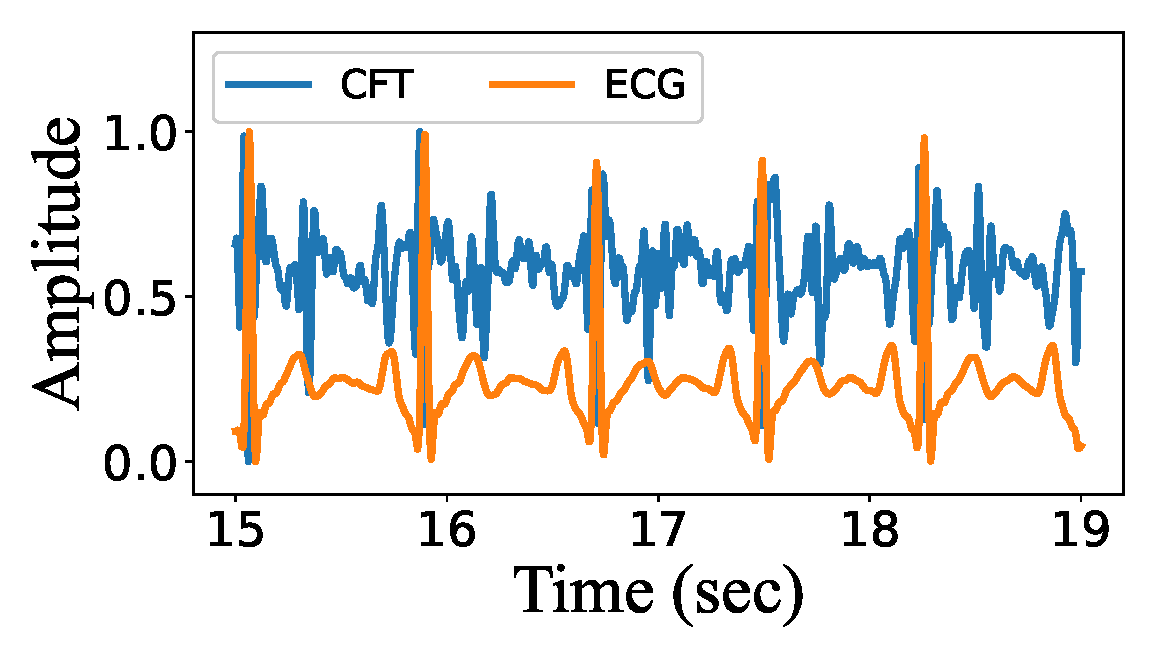
\includegraphics[width=0.3\columnwidth]{bf_good.eps}}
  \subfloat[]{\label{fig:MMECG_good}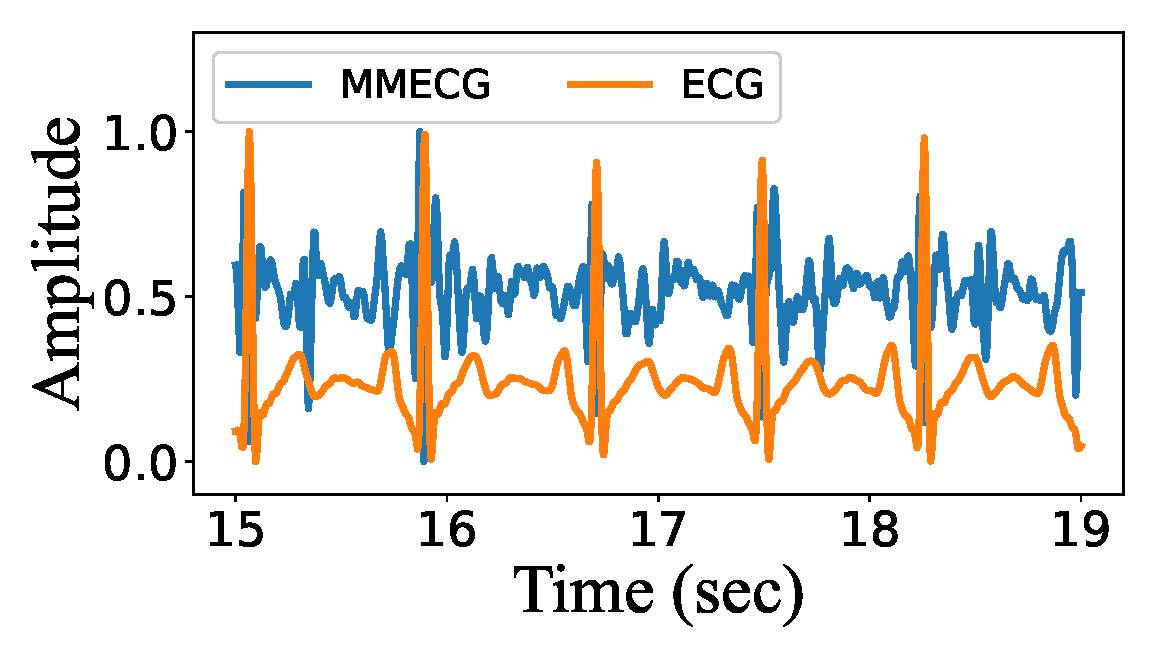
\includegraphics[width=0.3\columnwidth]{mmecg_good.eps}}
  \subfloat[]{\label{fig:vimo_good}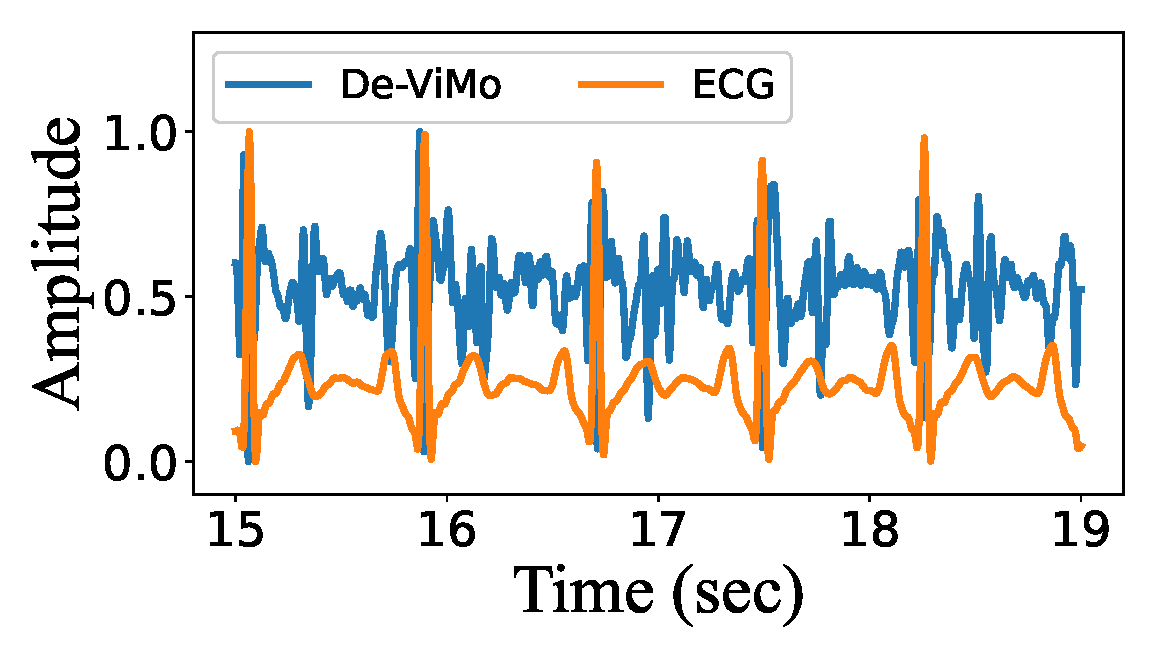
\includegraphics[width=0.3\columnwidth]{devimo_good.eps}}\\
\end{minipage}
\begin{minipage}{0.1\linewidth}\centering\scriptsize
\rotatebox[origin=center]{0}{\textbf{Rough Loc.}}
\rotatebox[origin=center]{0}{$\neq$}\\
\rotatebox[origin=center]{0}{\textbf{CF Point}}
\end{minipage}\begin{minipage}{0.9\linewidth}\centering
  \subfloat[]{\label{fig:bf_bad}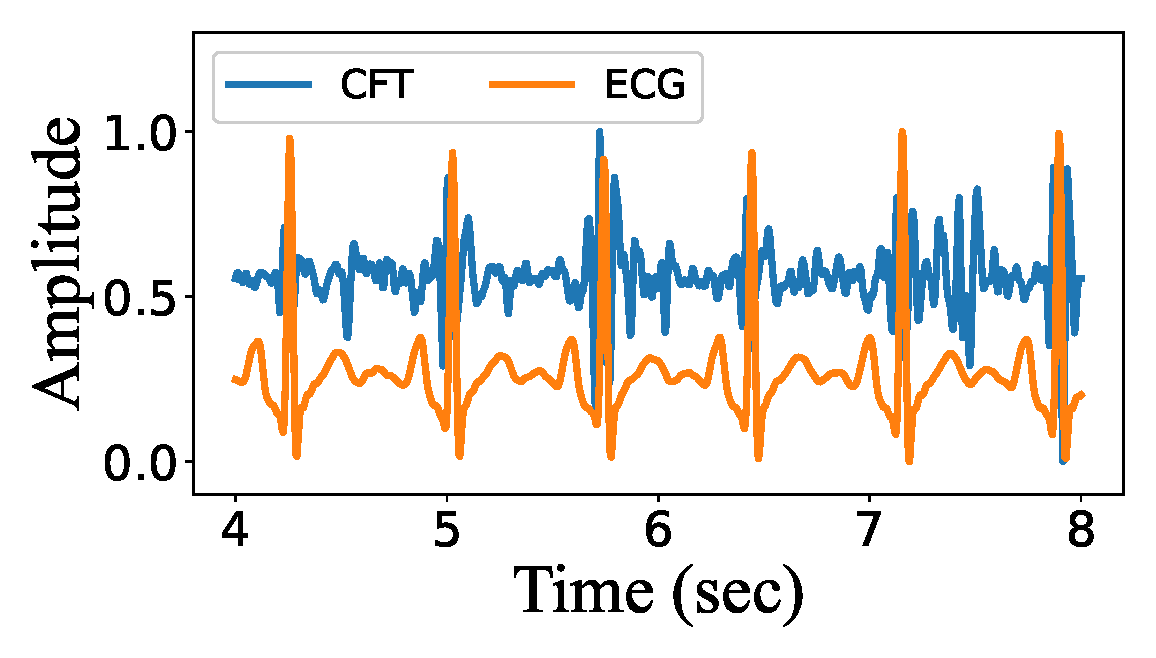
\includegraphics[width=0.3\columnwidth]{bf_bad.eps}}
  \subfloat[]{\label{fig:MMECG_bad}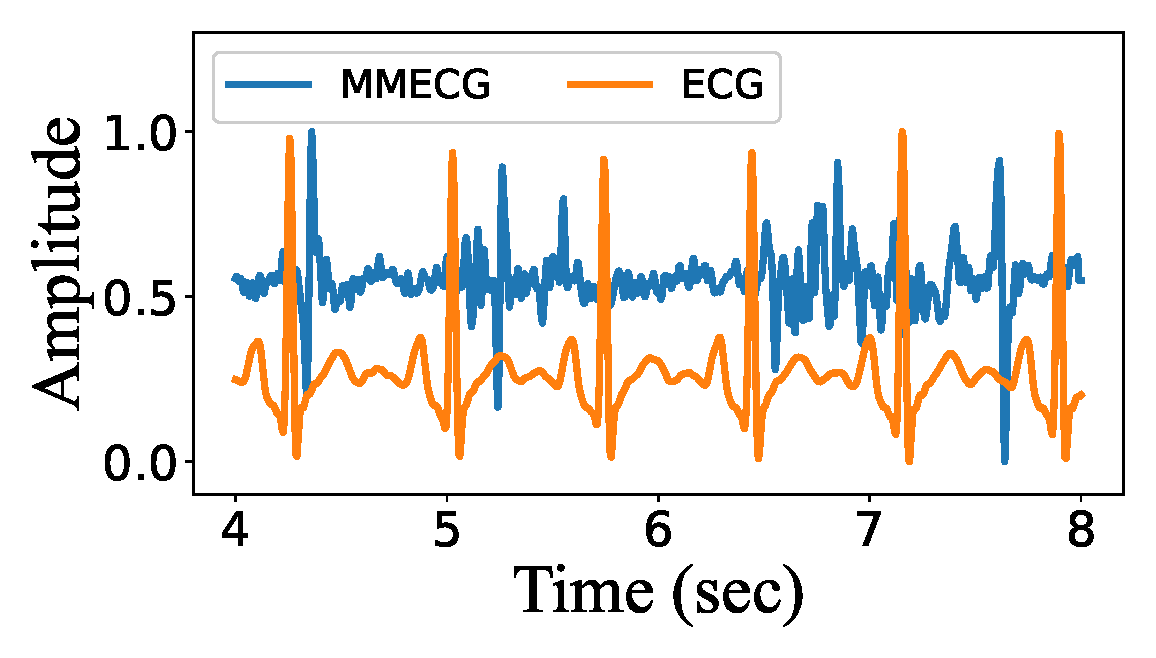
\includegraphics[width=0.3\columnwidth]{mmecg_bad.eps}}
  \subfloat[]{\label{fig:vimo_bad}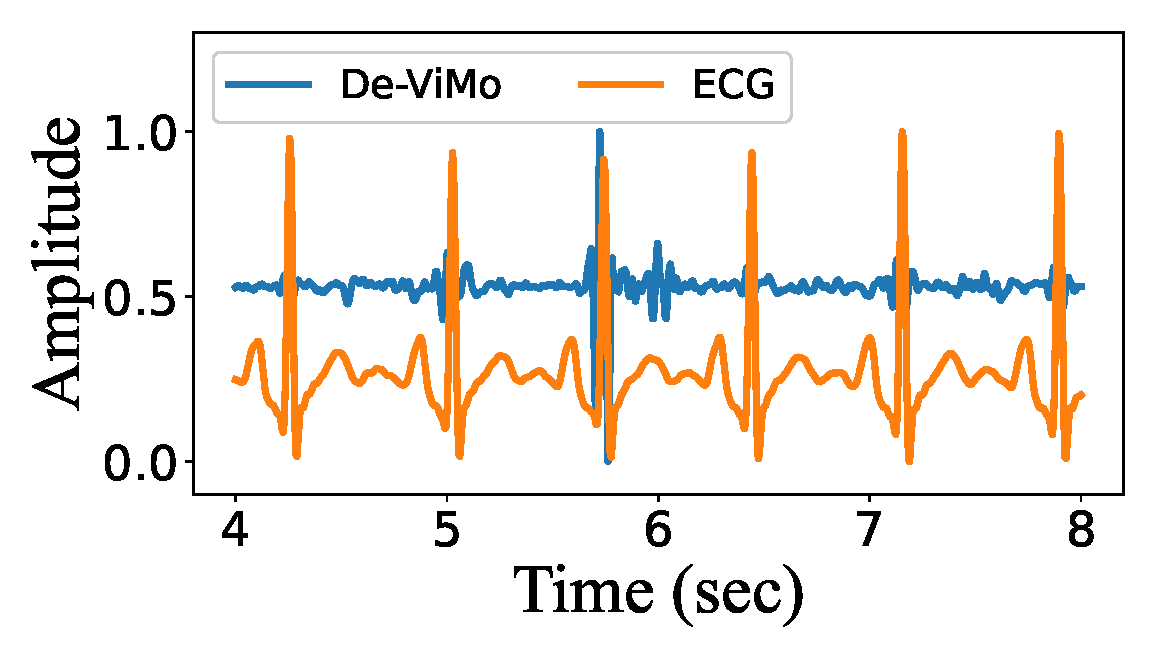
\includegraphics[width=0.3\columnwidth]{devimo_bad.eps}}
\end{minipage}
  \caption{Visualization of the extracted radar signal for all methods: (a) - (c) If CF point is around rough body location; (d) - (f) If CF point is far from rough body location.}
  \label{fig:compare_overall}
\end{figure*}

\section{Experimental Results and Evaluations}\label{sec:cftresult}
\subsection{Effectiveness of CFT Algorithm}
The examples of the extracted radar signal for different methods are shown in Figure~\ref{fig:compare_overall}, illustrating that precise cardiac localization has a huge effect on the signal quality. For example, if the rough body location is around CF point, all three methods can obtain high-SNR signals with clear first and second vibrations using either space search (CFT, Figure~\subref*{fig:bf_good}), clustering (MMECG, Figure~\subref*{fig:MMECG_good}) or accumulation (De-ViMo, Figure~\subref*{fig:vimo_good}). 

In contrast, only a few range bins will contain useful cardiac features if the rough body location is far from CF points, especially when increasing the monitoring range. Therefore, the signal accumulation may enhance the noises as shown in Figure~\subref*{fig:vimo_bad} while the signal clustering may also encounter a failure due to the lack of homogeneous cardiac signals as shown in Figure~\subref*{fig:MMECG_bad}. However, The proposed CFT could precisely locate the CF point with good SNR subject to the designed signal template and DFO searching strategy, and the extracted radar signal still shows clear peaks as shown in Figure~\subref*{fig:bf_bad}.

During the data collection of this study, the subjects are allowed to change postures to alleviate discomfort, with a resultant CF point deviation of several decimeters, while the rough location provided by FMCW signal processing is still unchanged. Therefore, the proposed CFT algorithm is essential because the posture change is inevitable, and a thorough evaluation in terms of different monitoring ranges will be performed in the next part.
\begin{figure}[tb]
  \centering
  \subfloat[]{\label{fig:pk_err_point}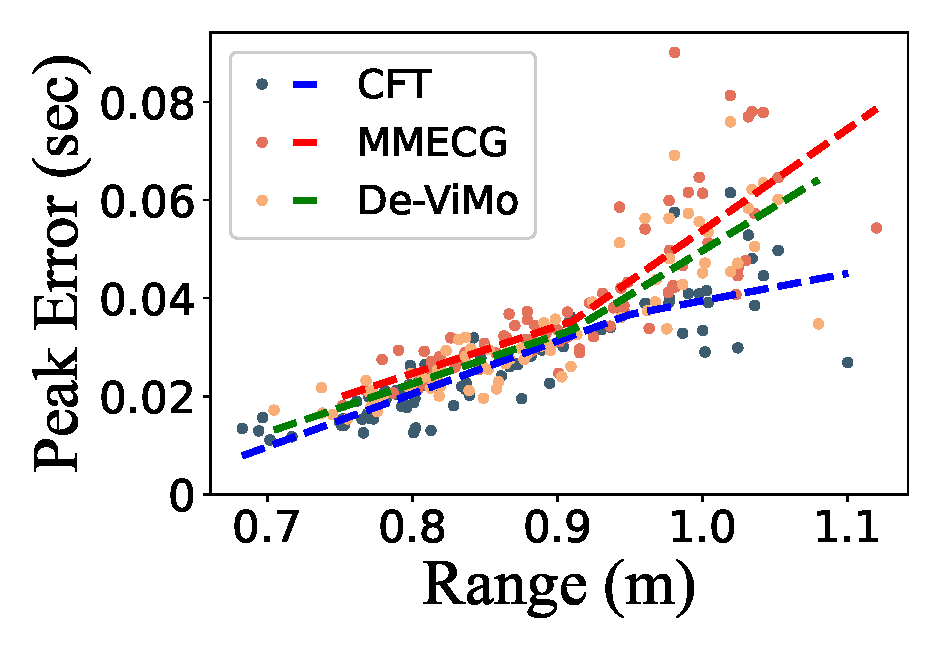
\includegraphics[width=0.35\columnwidth]{pk_err_point.eps}}
  \subfloat[]{\label{fig:pk_mdr_point}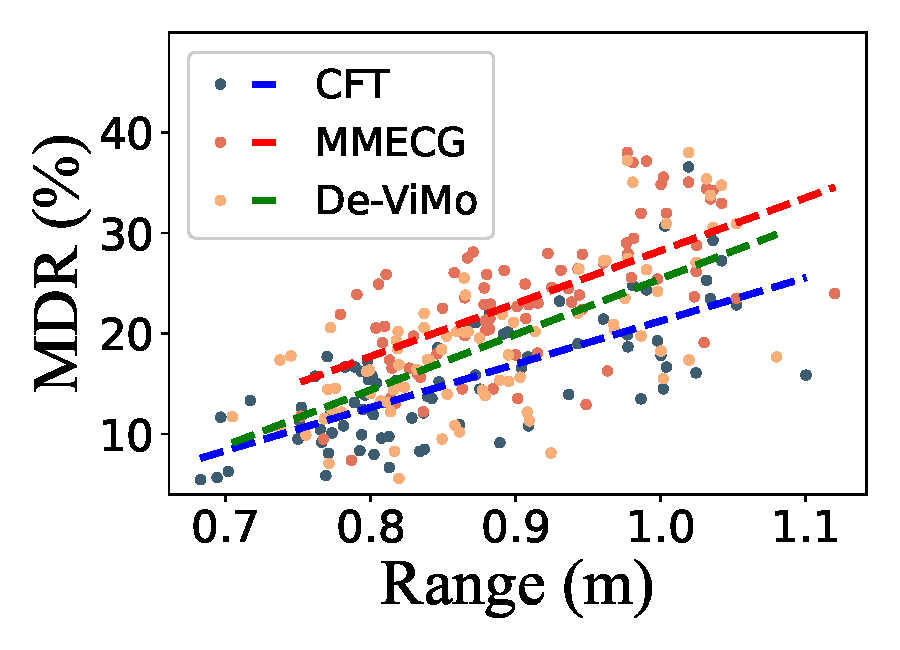
\includegraphics[width=0.34\columnwidth]{pk_mdr_point.eps}} \\
  \subfloat[]{\label{fig:pk_err_cdf}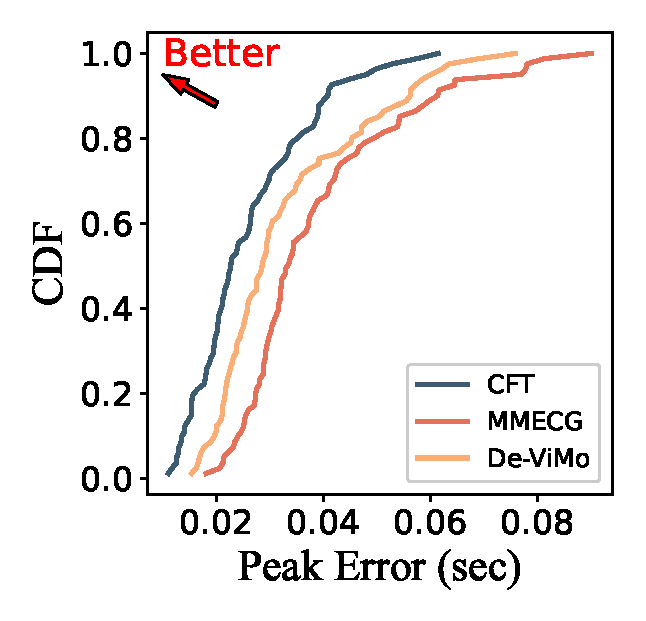
\includegraphics[width=0.35\columnwidth]{pk_err_cdf.eps}}
  \subfloat[]{\label{fig:pk_mdr_cdf}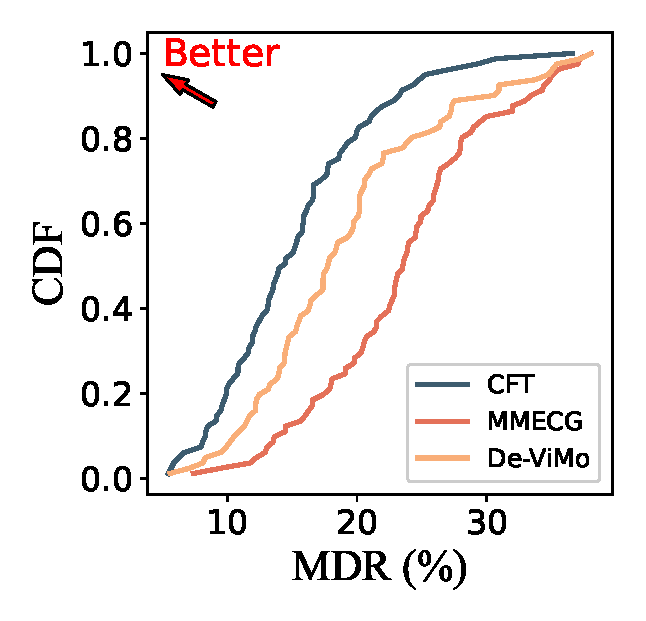
\includegraphics[width=0.35\columnwidth]{pk_mdr_cdf.eps}} 
  \caption{Illustration of performance in terms of peak error and MDR: (a) - (b) Scattered points with fitting curves along range axis; (c) - (d) CDF plots for all trails.}
  \label{fig:range_impact}
\end{figure}
\subsection{Impact of Monitoring Range}
To evaluate the performance of different methods when increasing the monitoring range, the quality of extracted radar signals for all trials is evaluated in terms of:
\begin{itemize}
\item Absolute Peak error between ECG R peaks and the dominant peaks for the first vibrations in radar signal.
\item \Gls{mdr} to count the cardiac cycles with no peak detected or with the absolute peak error larger than $150$ms~\cite{chen2022contactless}.
\end{itemize}

Figure~\subref*{fig:pk_err_point} and~\subref*{fig:pk_mdr_point} illustrate the peak error and MDR for all $80$ trials with corresponding fitting curves indicating the mean peak error or MDR. All the methods show similar performance in the short range and experience certain degradation with respect to the increasing range. In particular, MMECG shows larger degradation and variance for longer-range cases because the rough localization based on FMCW signal processing cannot provide accurate cardiac location, and the resultant evaluated points may not capture useful information for clustering. In contrast, De-ViMo could provide a better cardiac location, and the accumulated results show better accuracy than MMECG, while the long-range monitoring still affects the quality because the accumulation is not robust to non-gaussian noise. At last, the proposed CFT could precisely focus on the CF point and keep tracking the high-SNR points during data collection, providing the best results with small variance for both peak error and MDR. 

In addition, the \gls{cdf} plots for all trials are shown in Figure~\subref*{fig:pk_err_cdf} and~\subref*{fig:pk_mdr_cdf}. The proposed CFT algorithm achieves the best peak error with a median value of $0.022$~sec, while DE-ViMo and MMECG have worse performances with larger median values of $0.028$~sec and $0.033$~sec, respectively. Similarly, the precise localization and tracking of CF point also reduces the MDR for CFT results with a median value of $14\%$, while DE-ViMo and MMECG may affected by the accumulated noise or inaccurate cardiac localization with the median MDR of $17\%$ and $23\%$, respectively.


\subsection{Impact of Signal Quality on ECG Recovery}
The signals extracted using different methods are used for supervised training to verify the impact of different input qualities on the ECG recovery task. The quality of the recovered ECG signal is assessed in terms of:
\begin{itemize}
\item The morphological accuracy is measured using MSE and \Gls{pcc}, with MSE sensitive to the peak deviation and PCC focusing on the similarity between the ECG patterns.
\item The accurate recovery of ECG R peaks is crucial to coarse cardiac features calculation (e.g., heart rate variability) and is measured by absolute R peak error and MDR.
\end{itemize}
Table~\ref{tab:ecg_supervise} shows the performance of the deep learning model trained with datasets yielded by different methods. The training based on CFT dataset achieves the best results on both morphological accuracy (MSE$=0.0082$ and PCC$=85.47\%$) and R peak recovery (Peak Error$=7.61$ms and MDR$=6.85\%$), because the high-SNR inputs provide accurate peak locations with minor noise that affects the ECG pattern generation, as shown in Figure~\subref*{fig:radar_clean} and~\subref*{fig:ecg_pred_clean}. 

\begin{table}[tb]
\centering
\caption{Performance of supervised ECG recovery}
    \begin{tabular}{c |cccc}
    \toprule
    Methods  & \makecell[c]{MSE ($\times 10^{-2}$)} $\downarrow$ & PCC $\uparrow$ & \makecell[c]{Peak Error (ms)} $\downarrow$ & MDR $\downarrow$ \\
    \toprule
    MMECG~\cite{chen2022contactless} & $0.93$  & $80.36\%$ & $9.74$ & $7.96\%$ \\
    De-ViMo~\cite{liu2024diversity} & $0.88$ & $83.83\%$ & $8.93$ & $7.32\%$\\
    \midrule
    CFT  &  $\mathbf{0.82}$ & $\mathbf{85.47\%}$ & $\mathbf{7.61}$ & $\mathbf{6.85\%}$\\
    \bottomrule
    \end{tabular}%
\label{tab:ecg_supervise}
\end{table}%

In contrast, MMECG and De-ViMo cannot preserve the signal quality especially for long-distance cases, and the noisy inputs will prevent the deep learning mode from identifying the accurate position of ECG pieces, causing large peak error and MDR, as shown in Figure~\subref*{fig:radar_noise} and~\subref*{fig:ecg_pred_noise}. It is worth noticing that poor signal SNR causes more degradation in peak error than morphological accuracy, because the ECG patterns share a similar shape and can be learned from other cardiac cycles, while the peak recovery (detection) fully relies on the current radar input and can be ruined by noises.

\begin{figure}[tb]
  \centering
  \subfloat[]{\label{fig:radar_clean}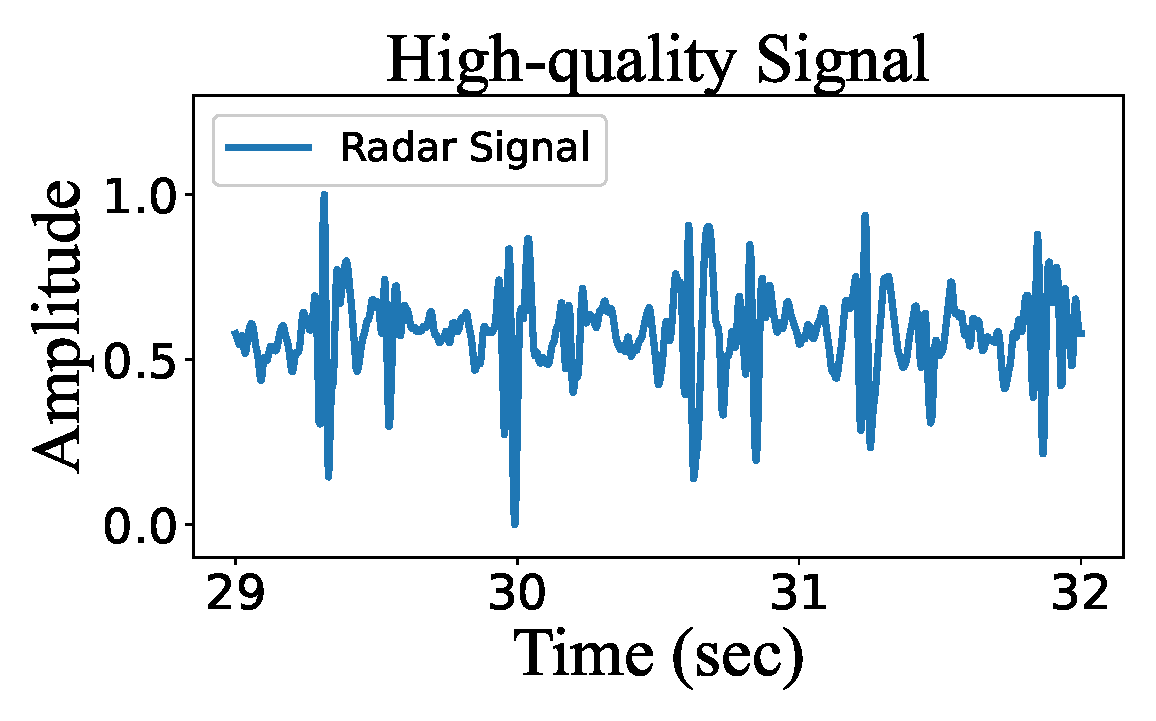
\includegraphics[width=0.4\columnwidth]{radar_clean.eps}}
  \subfloat[]{\label{fig:ecg_pred_clean}\includegraphics[width=0.4\columnwidth]{ecg_pred_clean.eps}} \\
  \subfloat[]{\label{fig:radar_noise}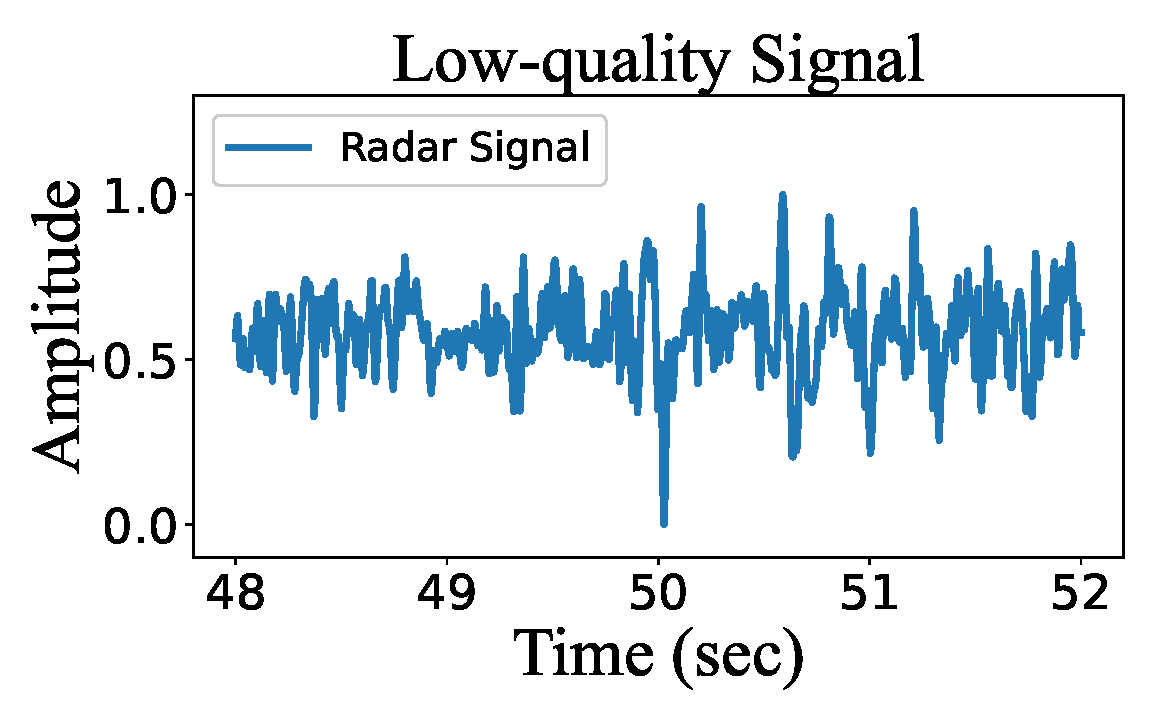
\includegraphics[width=0.4\columnwidth]{radar_noise.eps}}
  \subfloat[]{\label{fig:ecg_pred_noise}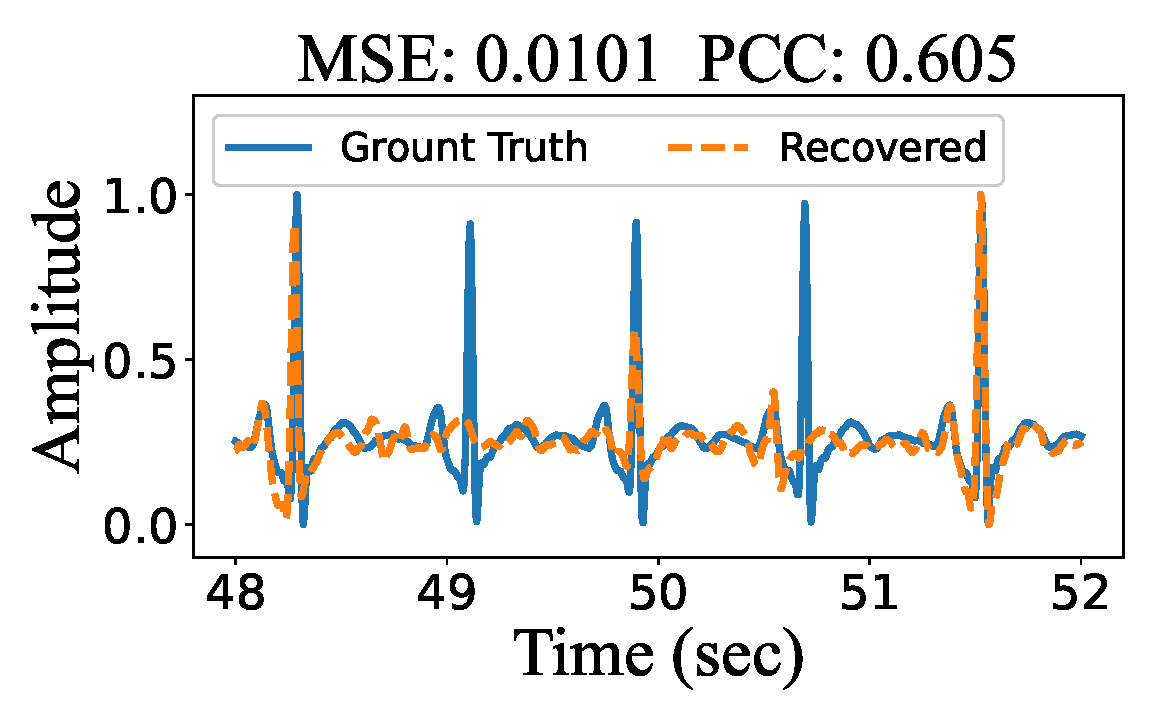
\includegraphics[width=0.4\columnwidth]{ecg_pred_noise.eps}} 
  \caption{Impact of radar input quality on the final ECG recovery: (a) - (b) High-quality radar input and ECG recovery; (c) - (d) Low-quality radar input and ECG recovery.}
  \label{fig:ecg_recovery}
\end{figure}

\section{Conclusions}\label{sec:cftcon}
This chapter investigates the efficient collection of high-SNR radar signals with ample cardiac features for deep-learning-based ECG recovery. Previous methods adopted signal accumulation or clustering to suppress the noises, while the rough localization based on FMCW radar cannot accurately reveal the chest region, requiring a time-consuming traverse among a 3D space for compensation. In this chapter, a novel CFT algorithm is proposed to dynamically articulate the points with the best SNR and could track the cardiac location over time if the subjects change posture. The experiments performed in different scenarios prove the feasibility of the CFT algorithm in radar signal collection for ECG recovery, enabling a convenient deployment in new scenarios for future contactless wellness monitoring.
